
\documentclass{article}
\usepackage[version=3]{mhchem} % Package for chemical equation typesetting
\usepackage{siunitx} % Provides the \SI{}{} and \si{} command for typesetting SI units
\usepackage[final]{graphicx}
\usepackage{natbib} % Required to change bibliography style to APA
\usepackage{amsmath} % Required for some math elements 
\usepackage{pythonhighlight}
\usepackage{commath}
\usepackage{listings}
\usepackage{xcolor}
\usepackage{gensymb}
\usepackage{subcaption}
\captionsetup[figure]{font=small,labelfont=small}
\usepackage{float}
\usepackage[margin=1in]{geometry}
\usepackage[hidelinks]{hyperref}
\hypersetup{
	colorlinks   = true, %Colours links instead of ugly boxes
	urlcolor     = blue, %Colour for external hyperlinks
	linkcolor    = blue, %Colour of internal links
	citecolor   = red %Colour of citations
}
\lstset { %
	language=C++,
	backgroundcolor=\color{black!5}, % set backgroundcolor
	basicstyle=\footnotesize,% basic font setting
}
\setlength\parindent{0pt} % Removes all indentation from paragraphs
\usepackage{hyperref}

\renewcommand{\labelenumi}{\alph{enumi}.} % Make numbering in the enumerate environment by letter rather than number (e.g. section 6)

%\usepackage{times} % Uncomment to use the Times New Roman font

%----------------------------------------------------------------------------------------
%	DOCUMENT INFORMATION
%----------------------------------------------------------------------------------------

\title{Implementation of a Raytracer \\ in C++ \\ Computer Graphics Lab (Rendering Track)} % Title

\author{Alhajras Algdairy \\alhajras.algdairy@gmail.com, 4963555, aa382} % Author name

\date{\today} % Date for the report

\begin{document}
	
	\maketitle % Insert the title, author, and date
	
	\begin{center}
		\begin{tabular}{l r}
			University: & University of Freiburg \\ % Date the experiment was performed
			Instructor: &Dr.-Ing. Matthias Teschner % Instructor/supervisor
		\end{tabular}
	\end{center}
	\clearpage
	% If you wish to include an abstract, uncomment the lines below
	% \begin{abstract}
	% Abstract text
	% \end{abstract}
	
	%----------------------------------------------------------------------------------------
	%	SECTION 1
	%----------------------------------------------------------------------------------------
	\tableofcontents
	\clearpage
	\section{Introduction}
	Computer graphics has three main pillars: \textit{Modelling}, \textit{Rendering}, and \textit{Simulation}. The focus of this report is Rendering. Rendering cares about solving issues like the model's visibility towards sensors; this is done by two methods: \textit{Rasterization} or \textit{Raytracing}, this report is about a Raytracer implementation. Rendering also focuses on which color and intensity does a model has. How light interacts with surfaces and how it propagates throw the media.
	
	The report summarizes the implementation of a simple Raytracer; this includes solving the Visibility challenge, coloring or shading the models and introducing some more features that enhance the Raytracer usability and performance.
	
	\vspace*{5px}
	Raytracing is a rendering technique that may provide extremely lifelike lighting effects. In other words, an algorithm can track the source of light and then mimic how the light interacts with the virtual objects it eventually encounters in the computer-generated environment. Raytracing produces far more lifelike shadows and reflections, as well as significantly enhanced translucence and dispersion. The algorithm considers where the light falls and calculates the interaction and interplay in the same way as the human eye does with actual light, shadows, and reflections. The way light interacts with items in the world has an impact on the colors you perceive.
	
	\vspace*{5px}
	Raytracer involves in different industries and applications. The media uses it because Raytracing can be beneficial in theater and television lighting since it allows for visually accurate simulation of light. Engineers also use the technique to forecast light levels, brightness gradients, and visual performance requirements in the following fields: Simulations, Modelling tools, and architectures. 
	
	\vspace*{5px}
    To render a scene by the Raytracer, three crucial steps must be followed: 
	\textit{Casting Rays}: cast a ray for each pixel in the image.
	\textit{Path tracing}: check if a ray crosses any of the scene's objects using the ray-geometry intersection, and trace the ray back to the source.
	\textit{Shading}: determine how the object looks (color and brightness) at the point where the ray intersects the object.
	
	\vspace*{5px}
	Raytracing has two main methods: 
	\begin{itemize}
		\item 		\textit{Forward Raytracing}: The light particles (photons) are tracked from the light source to the object via Forward Raytracing. While forward ray tracing is the most exact method for determining the color of each object, it is also the most inefficient.
		\item 		\textit{Backward Raytracing}: 
		An eye ray is formed at the eye in backward ray tracing, and it travels through the viewplane and out into the scene. If it hits an object, it will return it to the viewplane immediately. This method is more efficient than Forward Raytracing but less accurate due to reducing the rays used. In this implementation this method is used.
	\end{itemize}
	
	\clearpage
	%----------------------------------------------------------------------------------------
	%	SECTION 2
	%----------------------------------------------------------------------------------------
	\section{Visibility}
	\subsection{Introduction}
	The goal of rendering in computer graphics is to simulate light propagation to create images of virtual scenes. \textit{Visibility} is a critical phenomenon that occurs as a result of light's interaction with the environment.
	
	A fundamental graphics problem is determining the visible areas of surfaces and which object is closer to the camera. This challenge is referred to as visible surface determination or concealed surface removal, depending on how it is approached. The primary two operations in the Raytracer are Rays casting, which shoots rays toward the scene, and Path tracing that traces the path of the shooted rays.
	
	\subsection{Rays}
	To generate an image using Raytracing, we must first cast a ray for each pixel in the image to the scene.
	Raytracing is a computer approach for simulating the behavior of light in a three-dimensional scene. It works by replicating genuine light rays and tracing the path that a beam of light would travel in the real environment using an algorithm. 
	For this, all raytracers use rays as a way to simulate photons. Let us think of a ray as a function; here $\pmb{r} $ is a 3D position along a line in 3D. $\pmb{o} $ is the ray origin and $\pmb{d} $ is the ray direction.
	\begin{equation}
		\pmb{r} (t) = \pmb{o} + t\pmb{d} ,  \quad  0 < t < \infty
	\end{equation}
	
	Figure ~\ref{fig:1} shows the basic idea of raytracing, where several rays are shooted toward the scene, and then a path tracer algorithm is used to shade the object and detect which parts are visible to the camera.
	\begin{figure}[H]
		\begin{center}
			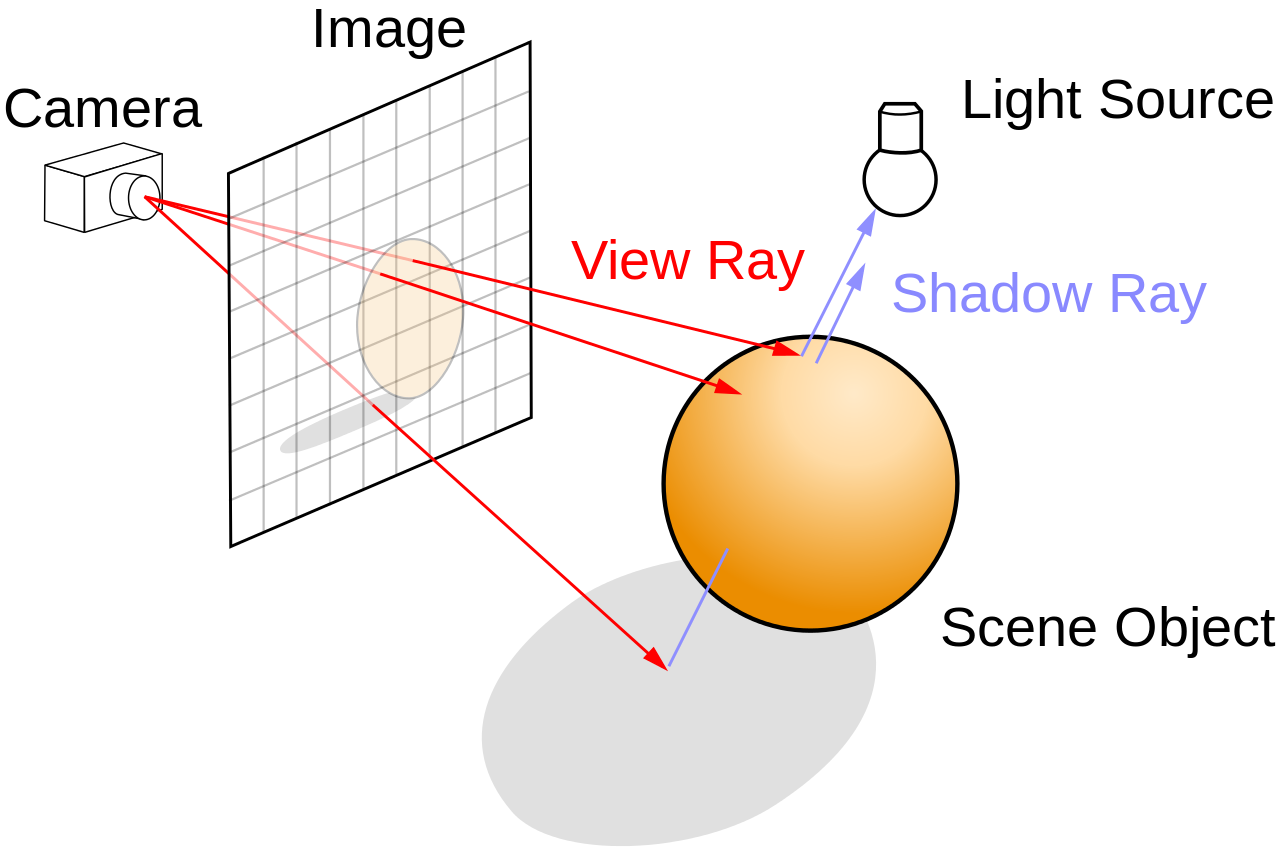
\includegraphics[width=250pt]{C:/D/University/Semester_4/Raytracer/lab_report_1/assignment_2/images/3.png}
			
			\caption{The raytracing algorithm builds an image by extending rays into a scene and bouncing them off surfaces and towards sources of light to approximate the color value of pixels [Piotr Dubla, "Interactive Global Illumination on the CPU."
				]}
			\label{fig:1}
		\end{center}
	\end{figure}
	
	\subsection{Rendering a Sphere}
	For testing, spheres are often used in ray tracers because
	calculating whether a ray hits a sphere is pretty straightforward.
	
	The general equation of a sphere with radius = 1 is:
	\begin{equation}
		(o_x + td_x )^2 + (o_y + td_y )^2+ (o_z + td_z )^2= 1
	\end{equation}
	
	For solving the equation we need to use the Quadratic equation in t: 
	
	\begin{equation}
		\begin{split}
			A(t)^2 + Bt+ C= 0 \\
			A = d^2_x + d^2_y + d^2_z \\	
			B = 2(d_xo_x + d_yo_y + d_zo_z) \\
			C = o^2_x + o^2_y + o^2_z - 1 \\
			t_{1,2} = \frac{-B \pm \sqrt{B^2 - 4AC}}{2A}\\
		\end{split}		
	\end{equation}
	
	
	By solving the equation we get three different cases as shown in Figure ~\ref{fig:2}:
	
	\begin{itemize}
		\item No Intersection if: \( B^2 - 4AC < 0 \) 
		\item Single point of intersection if: \( B^2 - 4AC = 0 \)
		\item Otherwise we get two points of intersection
	\end{itemize}
	
	
	\begin{figure}[H]
		\begin{center}
			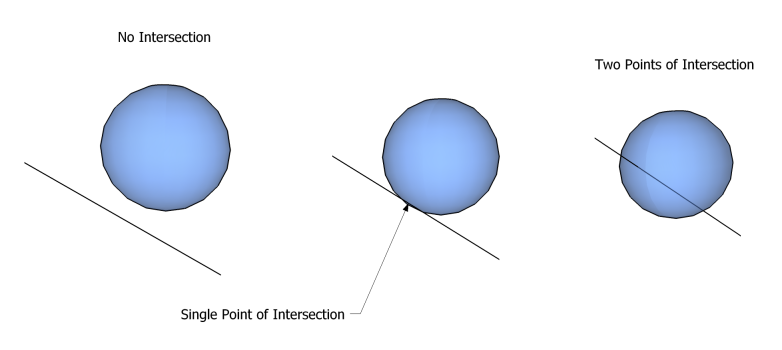
\includegraphics[width=250pt]{C:/D/University/Semester_4/Raytracer/lab_report_1/assignment_2/images/5.png}
			
			\caption{The three possible line-sphere intersections:
				1. No intersection.
				2. Point intersection.
				3. Two point intersection.}
			\label{fig:2}
		\end{center}
	\end{figure}
	
	\subsection{Rendering Triangle}
	It is computing the intersection of a ray with a primitive such as a sphere is not tricky. However, because modeling most 3D objects with spheres alone is difficult, other types of primitives must be used to represent more complicated objects (objects of arbitrary shape).
	We may transform every object into a triangular mesh and compute the intersection of a ray with every triangle in this mesh instead of working with complex primitives like NURBS or Bezier patches.
	We get three different cases by solving the equation as shown in Figure ~\ref{fig:3} below.
	
	Parametric representation:
	\begin{equation}
		\begin{split}
			\pmb{p}(b_1,b_2) = (1 - b_1 - b_2)\pmb{p}_0 + b_1\pmb{p}_1 + b_2\pmb{p}_2\\
		\end{split}		
	\end{equation}
	Vertices $\pmb{p}_0$, $\pmb{p}_1$, $\pmb{p}_2$ form a triangle. $\pmb{p}$ is an arbitrary point in the plane
	of the triangle.
	
	Figure ~\ref{fig:3} shows the three different cases that the ray can have with a triangle: Ray misses, Ray parallel and the one we are interested in is when the ray intersects, we get an intersection if: 
	\( b_0 \geq
	0 \land b_1\geq
	0 \land b_2 \geq
	0 \)
	
	
	
	\begin{figure}[H]
		\begin{center}
			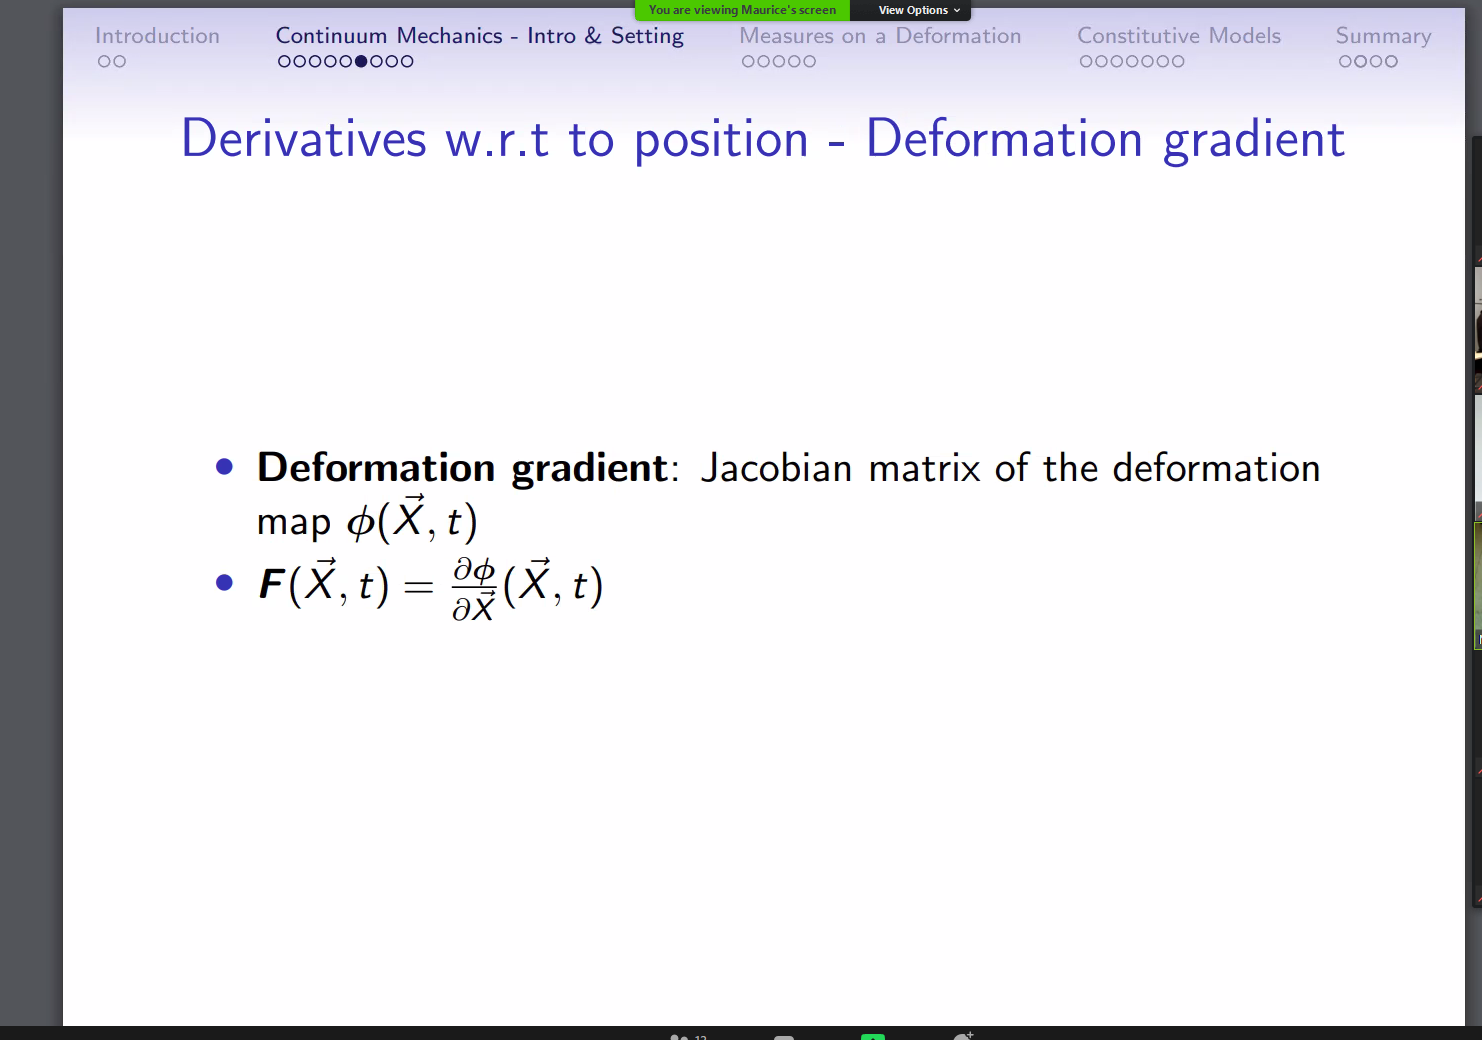
\includegraphics[width=250pt]{C:/D/University/Semester_4/Raytracer/lab_report_1/assignment_2/images/9.png}
			
			\caption{Three cases of ray intersect with a triangle.}
			\label{fig:3}
		\end{center}
	\end{figure}
	
	\subsection{Anti-aliasing}
	Pixels make up the display on a computer. The smallest component of any digital image is the pixel, and while modern computer monitors have great resolutions with millions of pixels, these pixels are still rectangular. This means that when spherical forms are displayed on a screen, the user will almost certainly notice jagged edges, also known as aliasing.
	We'll utilize a basic MSAA, which stands for "multisample anti-aliasing" and is one of the most prevalent anti-aliasing techniques. It achieves the finest blend of visual accuracy and performance in most cases. This is done by averaging the number of samples within each pixel.
	
	We have several samples within that pixel for a given pixel and send rays through each of the samples. The colors of these rays are then averaged.
	
	\begin{figure}[ht]
		\begin{center}
			\begin{subfigure}{.3\textwidth}
				\centering
				% include first image
				
\includegraphics[width=.8\linewidth]{C:/D/University/Semester_4/Raytracer/lab_report_1/assignment_2/images/without_aa.png}  
				\caption{Alising}
				\label{fig:sub-first}
			\end{subfigure}
			\begin{subfigure}{.3\textwidth}
				\centering
				% include second image
				
\includegraphics[width=.8\linewidth]{C:/D/University/Semester_4/Raytracer/lab_report_1/assignment_2/images/with_aa_100.png}  
				\caption{Anti-aliasing with 100 samples per pixel}
				\label{fig:sub-second}
			\end{subfigure}
			
			\caption{he benefit of using Anti-aliasing improvement, where (b) looks smoother than (a)}
			\label{fig:4}
		\end{center}
	\end{figure}
	
	
	Figure ~\ref{fig:4} shows the refinement and how the object's edges are smoothed by using the anti-aliasing technique. The issue is performance because the more smoothed edges get, the more samples had to be taken around each pixel; for example, if the image size is 200 x 200, and the samples are used for anti-aliasing are equal to 100, then we will measure the color for 200 x 200 x 100 pixels rather than 200 x 200. 
	A trade-off has to be done here in order to have a smoothed edges, but with no considerable performance cost; this depends on the application. 
	
	
	\subsection{Implementation}
	Two classes of Sphere and Triangle are created; each class or model contains parameters depending on its shape. Also, each model needs a different intersection test, as explained before. 
	After casting rays toward the scene, it will loop over all the objects in the scene and test the intersection; if the ray intersects an object, it will save its position and color of the pixel if there is no object intersect closer to the previous object, we just return the color of the pixel. 
	For more complicated objects as a cube, an array or mesh of triangles is arranged in a specific position to compose a cube. This mesh is an object called a cube, but it is composed of triangles; hence the triangle intersection test is being used.
	
	For anti-aliasing, there is a configuration class that contains the global settings for the Raytracer, and one configuration is the number of samples used for the anti-aliasing.
	
	
	\subsection{Results and discussion}
	
	There are so many formats for images, we will be using PPM file to save the output of the scene. Figure ~\ref{fig:5} shows different shapes that rendered. Spheres are good models for testing the lights and shading performance, Triangles are helpful in order to create meshes out of them as shown in (c) where a cube is rendered by adding 12 triangles. 
	\begin{figure}[ht]
		\begin{center}
			\begin{subfigure}{.3\textwidth}
				\centering
				% include first image
				\includegraphics[width=.8\linewidth]{C:/D/University/Semester_4/Raytracer/lab_report_1/assignment_2/images/6_2.png}  
				\caption{Rendering a simple Sphere}
				\label{fig:sub-first}
			\end{subfigure}
			\begin{subfigure}{.3\textwidth}
				\centering
				% include second image
				\includegraphics[width=.8\linewidth]{C:/D/University/Semester_4/Raytracer/lab_report_1/assignment_2/images/7_2.png}  
				\caption{Rendering a simple Triangle}
				\label{fig:sub-second}
			\end{subfigure}
			\begin{subfigure}{.3\textwidth}
				\centering
				% include second image
				\includegraphics[width=.8\linewidth]{C:/D/University/Semester_4/Raytracer/lab_report_1/assignment_2/images/cube.png}  
				\caption{Rendering a cube made out of triangles mesh}
				\label{fig:sub-third}
			\end{subfigure}
			
			\caption{Rendering different shapes in the scene}
			\label{fig:5}
			
		\end{center}
	\end{figure}
	
	\textbf{Resources and further reading}: 
	Most material and code used in this chapter is mixed between the book [Peter Shirley. 	\textit{"Ray Tracing in One Weekend"}] and the slides 		[Matthias Teschner, 	\textit{"Advanced Computer Graphics"}].
	
	
	\clearpage
	
	%----------------------------------------------------------------------------------------
	%	SECTION 3
	%----------------------------------------------------------------------------------------
	
	
	
	\section{Shading}
	\subsection{Introduction}
	
	Rendering a scene needs two steps; the first step is solving the visibility issue, which means which object is visible to the camera and what its shape is. The second step is Shading, and this deals with the color of the object and its intensity. Shading also includes how object's color affects each other; for example, having light hits, the object will make its color look brighter; on the other hand, regions in which light does not hit or reach will have dark color or shadow. In this chapter, shading concepts will be discussed and implemented.  The primary key to Shading is calculating the amount of light that hits a point; let us call it P. 
	
	The computed light at a point P depends on the following: 
	
	\begin{itemize}
		\item Light illuminated by source source  $\pmb{L}^{source}$  in real life usually lamp, fire or the sun, it can have any color and intensity but here we will use white color. 
		\item Surface illumination $\pmb{L}^{surface}$.
		\item Light reflected from the surface $\pmb{L}^{reflected}$.
		\item The observation angle / looking at angle / camera. 
	\end{itemize}
	
	
	
	
	\subsubsection{Lambert's Cosine Law}
	The amount of light energy arriving at a surface is proportional to the cosine of the angle between the light direction and the surface normal, according to Lambert's cosine law. Illumination strength at a surface is proportional to the cosine of the angle between $\pmb{l}$ and $\pmb{n}$, the angel will be denoted as $\theta$, the following three cases illustrate the relationship between the  $\pmb{L}^{source}$ and  $\pmb{L}^{surface}$:
	
	The  $\pmb{L}^{surface}$,$ \pmb{L}^{source}$ relation is: $\pmb{L}^{surface} = \pmb{L}^{source}.\cos \theta $
	\begin{itemize}
		\item $\pmb{L}^{surface} = \pmb{L}^{source}$, if $\theta = 0\degree$.
		\item $\pmb{L}^{surface} = 0$, if $\theta = 90\degree$.
		\item $0 < \pmb{L}^{surface} < \pmb{L}^{source}$, if $0\degree < \theta  < 90\degree$.
	\end{itemize}
	
	\subsubsection{Phong reflection model }
	Phong reflection is a model of local illumination. It defines how light reflects off a surface as a mixture of diffuse reflection from rough surfaces and specular reflection from polished surfaces. It's based on Phong's intuitive observation that bright surfaces have small, strong specular highlights, and dull surfaces have larger, more gradual specular highlights. nThe model also includes an ambient term to account for the small amount of light that is scattered about the entire scene.
	\\
	
	\begin{itemize}
		\item \pmb{Ambient reflection}
		\begin{equation}
			\pmb{L}^{amb} = \pmb{\rho}\otimes \pmb{L}^{indirect}
		\end{equation}
		
		\begin{itemize}
			\item $\pmb{\rho}$, is the surface color
			\item $\pmb{L}^{indirect}$ , is the light reflected from other surfaces and objects, excluded the direct light ($\pmb{L}^{source}$)
		\end{itemize}
		\item \pmb{Diffuse reflection} 
		
		\begin{equation}
			\pmb{L}^{diff} =  \pmb{L}^{source}.(\pmb{n}.\pmb{l}) \otimes \pmb{\rho} 
		\end{equation}
		\begin{itemize}
			\item $\pmb{L}^{source}$, is the light source color and intensity which usually white. 
			\item $\pmb{n}$ and $\pmb{l}$ , are the representation of the Lambert's cosine law, where n is the normal surface vector  and l is the indecent light coming from the light source.
		\end{itemize}
		\item \pmb{Specular reflection} 
		
		\begin{equation}
			\pmb{L}^{spec} =  \pmb{L}^{source}.(\pmb{n}.\pmb{l}).(\pmb{r}.\pmb{v})^m \otimes \pmb{\rho}^{white} 
		\end{equation}
		\begin{itemize}
			\item $\pmb{r}$, which is the direction that a perfectly reflected ray of light would take from this point on the surface. 
			\item $\pmb{v}$, which is the direction pointing towards the viewer (such as a virtual camera).
			\item $m$, which is a shininess constant for this material, which is larger for surfaces that are smoother and more mirror-like. When this constant is large the specular highlight is small.
		\end{itemize}
	\end{itemize}
	
	The overall illumination on the surface can be computed by summing up the three components that make up \textit{Phong model}:
	
	\begin{equation}
		\pmb{L}^{surface}= \pmb{L}^{amb} + \sum_{n=1}^{lights} (\pmb{L}_n^{diff} + \pmb{L}_n^{spec})
	\end{equation}
	
	
	\begin{figure}[ht]
		\begin{center}
			\begin{subfigure}{.3\textwidth}
				\centering
				% include first image
				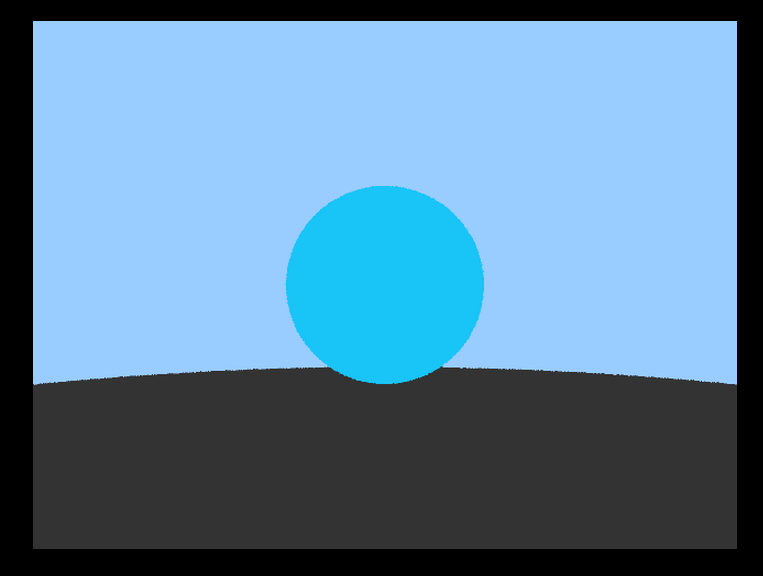
\includegraphics[width=.8\linewidth]{C:/D/University/Semester_4/Raytracer/lab_report_1/assignment_2/images/amb_reflection.png}  
				\caption{Ambient}
				\label{fig:sub-first}
			\end{subfigure}
			\begin{subfigure}{.3\textwidth}
				\centering
				% include second image
				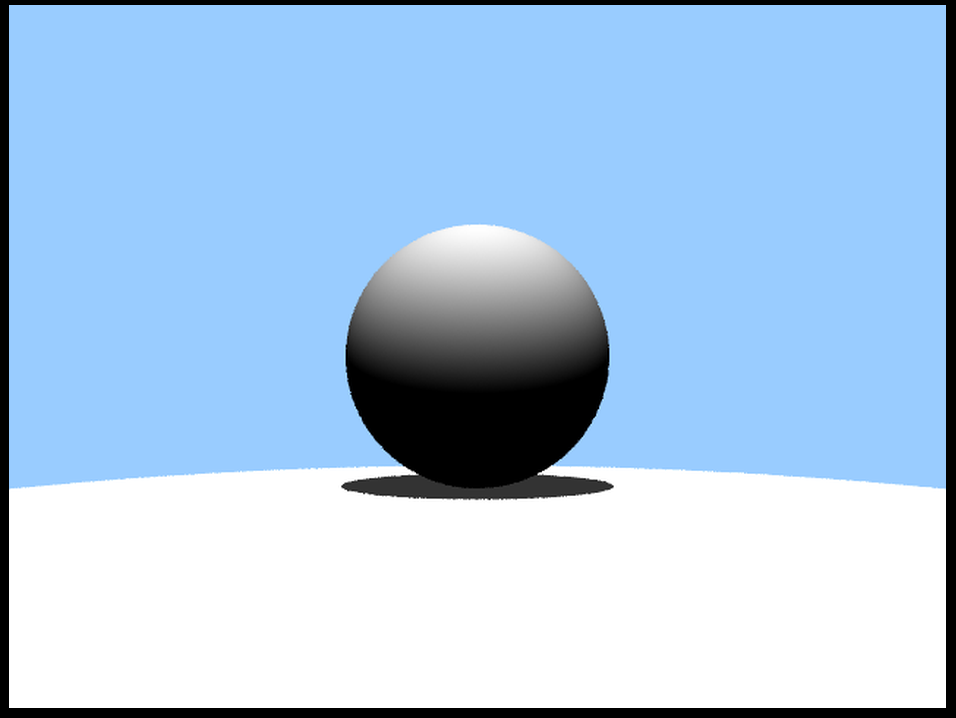
\includegraphics[width=.8\linewidth]{C:/D/University/Semester_4/Raytracer/lab_report_1/assignment_2/images/diff_reflection_2.png}  
				\caption{Diffuse}
				\label{fig:sub-second}
			\end{subfigure}
			\begin{subfigure}{.3\textwidth}
				\centering
				% include second image
				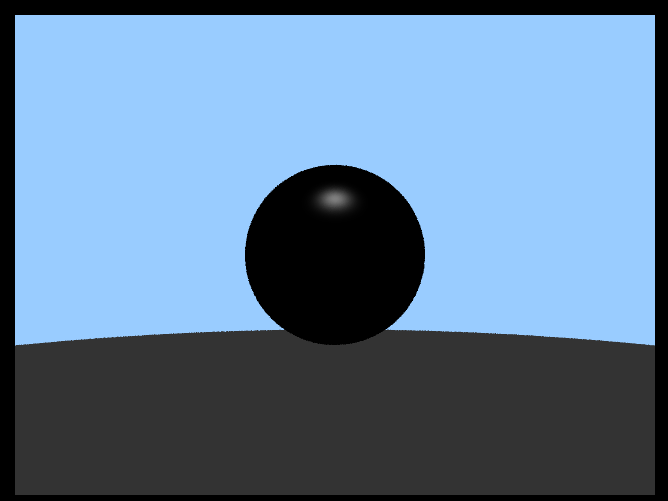
\includegraphics[width=.8\linewidth]{C:/D/University/Semester_4/Raytracer/lab_report_1/assignment_2/images/spec_reflection_2.png}  
				\caption{ Specular (Glossy)}
				\label{fig:sub-third}
			\end{subfigure}
			
			\caption{Visual illustration of the Phong equation}
			\label{fig:6}
		\end{center}
	\end{figure}
	
	\subsubsection{Results and discussion}
	
	Figure ~\ref{fig:7} shows the result of using a Phong model to shade a Sphere in a scene. (a) shows the $\pmb{L}^{amb}$ only. (b) represents the $\pmb{L}^{amb}$ and $\pmb{L}^{diff}$, (c) shows the overall light calculated from the scene $\pmb{L}^{amb}$, $\pmb{L}^{diff}$ and $\pmb{L}^{spec}$, (d) illustrated the summation of two different light sources for the $\pmb{L}^{diff}$ and $\pmb{L}^{spec}$ that is why the scene is brighter, two shadows for the Sphere and also two specular points on the Sphere.
	\begin{figure}[H]
		\begin{center}
			\begin{subfigure}{.3\textwidth}
				\centering
				% include first image
				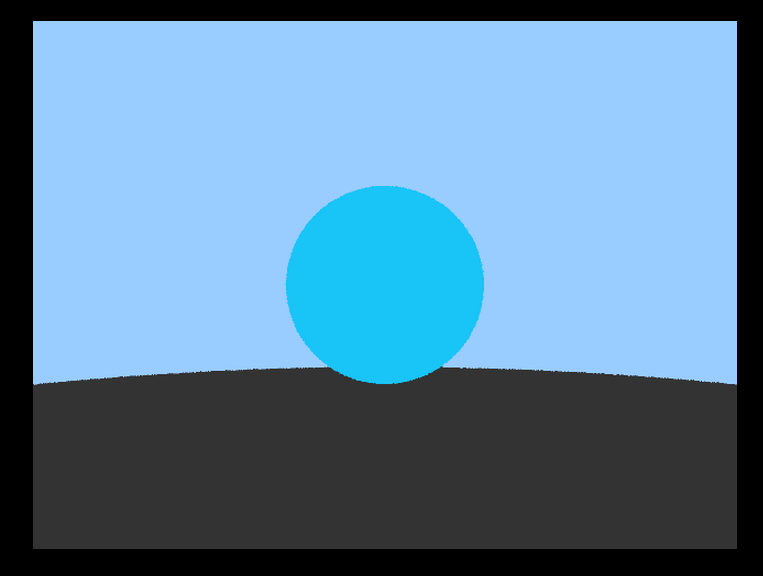
\includegraphics[width=.8\linewidth]{C:/D/University/Semester_4/Raytracer/lab_report_1/assignment_2/images/amb_reflection.png}  
				\caption{Ambient}
				\label{fig:sub-first}
			\end{subfigure}
			\begin{subfigure}{.3\textwidth}
				\centering
				% include second image
				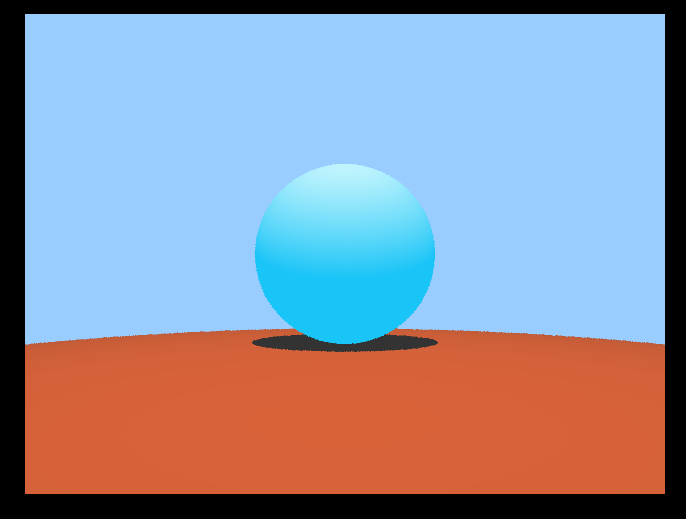
\includegraphics[width=.8\linewidth]{C:/D/University/Semester_4/Raytracer/lab_report_1/assignment_2/images/diff_reflection.png}  
				\caption{Diffuse + Ambient}
				\label{fig:sub-second}
			\end{subfigure}
			\begin{subfigure}{.3\textwidth}
				\centering
				% include second image
				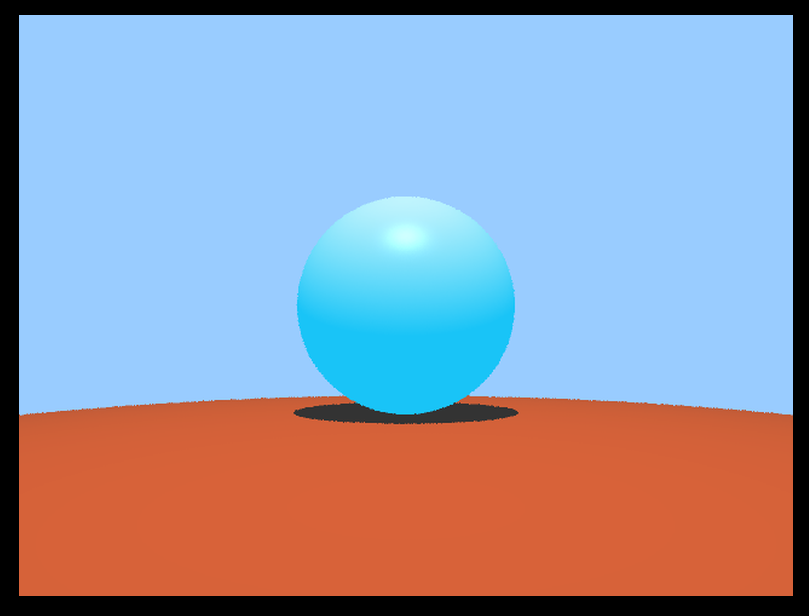
\includegraphics[width=.8\linewidth]{C:/D/University/Semester_4/Raytracer/lab_report_1/assignment_2/images/spec_reflection.png}  
				\caption{Diffuse + Ambient + Specular (Glossy)}
				\label{fig:sub-third}
			\end{subfigure}
			
			\begin{subfigure}{.3\textwidth}
				\centering
				% include second image
				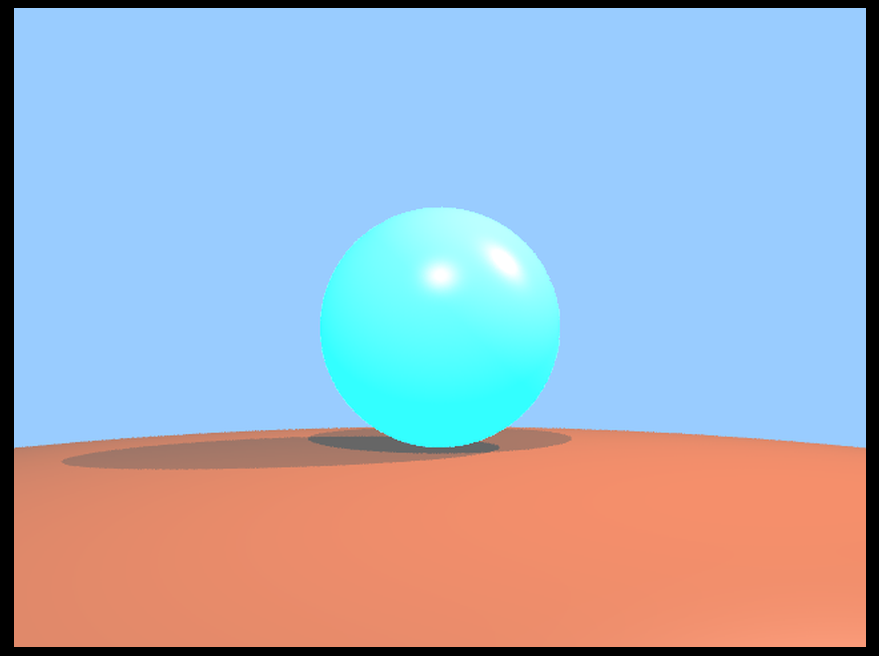
\includegraphics[width=.8\linewidth]{C:/D/University/Semester_4/Raytracer/lab_report_1/assignment_2/images/multi_shadow_multi_spec.png}  
				\caption{Multiple lights that generates brighter surface and multiple shadows}
				\label{fig:sub-third}
			\end{subfigure}
			\caption{Using a Phong model to shade a sphere.}
			\label{fig:7}
		\end{center}
	\end{figure}
	
	
	\subsection{Materials}
	
	In Raytracing, one of the important topics is to give the object a material type, and this can be: Glossy, Diffuse, Transparent, and Subsurface
	scattering, each material has different surface reflection and refraction properties, some surfaces reflect the light equally such as diffuse surfaces, some are reflecting light into a dominant direction as Glossy surfaces, some material such as water will reflect some light but also refract some.
	\\ 
	In the previous chapter, we discussed diffuse and specular (Glossy) surfaces. In this chapter, we will implement a refraction surface because it has interesting properties. 
	
	\subsubsection{Refraction}
	The refraction phenomenon happens when the light passes from one medium to a different medium.
	Figure ~\ref{fig:refraction} illustrates this phenomenon, $I$ is the incident light ray, $R$ is the reflected light where $N$ is the normal vector to the surface which is water (in blue), the reflected angle  $\theta2$ is equal to the incident angle $\theta1$, in addition to the reflected light there is a refracted light $T$, the direction of $T$ depends on the $\theta1$ and \textit{refractive index, $\eta$} ( Describes how fast light travels through the material).
	
	The ratio of the sines of the angle of incidence  $\theta1$ and angle of refraction $\theta2$ is equivalent to the opposite ratio of the indices of refraction for a particular pair of media, according to \textit{Snell's law}:
	
	
	\begin{equation}
		\frac{sin(\theta_1)}{sin(\theta_2)} = \frac{\eta_2}{\eta_1} 
	\end{equation}
	
	
	\begin{figure}[H]
		\begin{center}
			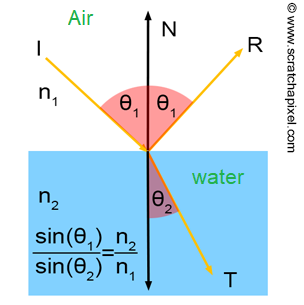
\includegraphics[width=150pt,height=150pt]{C:/D/University/Semester_4/Raytracer/lab_report_1/assignment_2/images/refraction.png}
			
			\caption{Incident light $I$ in the air hitting water surface, $R$ is reflected light and $T$ is the transmitted and refracted light, $n$ is \textit{refractive index, $\eta$  } Resource: \href{https://www.scratchapixel.com/images/upload/shading-intro/shad-refraction6.png?}{scratchapixel.com}.
				]}
			\label{fig:refraction}
		\end{center}
	\end{figure}
	
	\subsubsection{Fresnel}
	The amount of light that is reflected vs. refracted can be calculated using what is known as the \textit{Fresnel equations}, where $F_R$ is the reflected light portion, and $F_T$ is the portion transmitted through the material. 
	
	\begin{equation}
		F_R = \dfrac{1}{2}(\left( \dfrac{\eta_2 \cos\theta_1 - \eta_1 \cos \theta_2}{\eta_2 \cos\theta_1 + \eta_1 \cos \theta_2} \right)^2 + \left( \dfrac{\eta_1 \cos\theta_2 - \eta_2 \cos \theta_1}{\eta_1 \cos\theta_2 + \eta_2 \cos \theta_1} \right)^2)
	\end{equation}
	
	
	
	\begin{equation}
		F_T= 1 - F_R 
	\end{equation}
	
	\subsubsection{Texture}
	A texture can be uniforms, such as a brick wall, or irregulars, such as wood grain or marble. The conventional way is to build a "texture map," which is a 2D bitmapped picture of the texture that is then "wrapped around" the 3D object. Instead of using bitmaps, another option is to compute the texture entirely using mathematical models. Textures are so helpful; they reduce the geometric complexity of a scene by mapping a bit directly to an image or having a mathematical equation that can easily represent the surface color, they also reduce the number of vertices, and it reduces the modeling and rendering time. 
	
	Procedural texturing describes ways to employ texture values, such as replacing the original surface color with the texture color linearly combining the original surface color with the texture multiply, add, subtract surface color and texture color.
	
	
	\begin{figure}[ht]
		\begin{center}
			\begin{subfigure}{.3\textwidth}
				\centering
				% include first image
				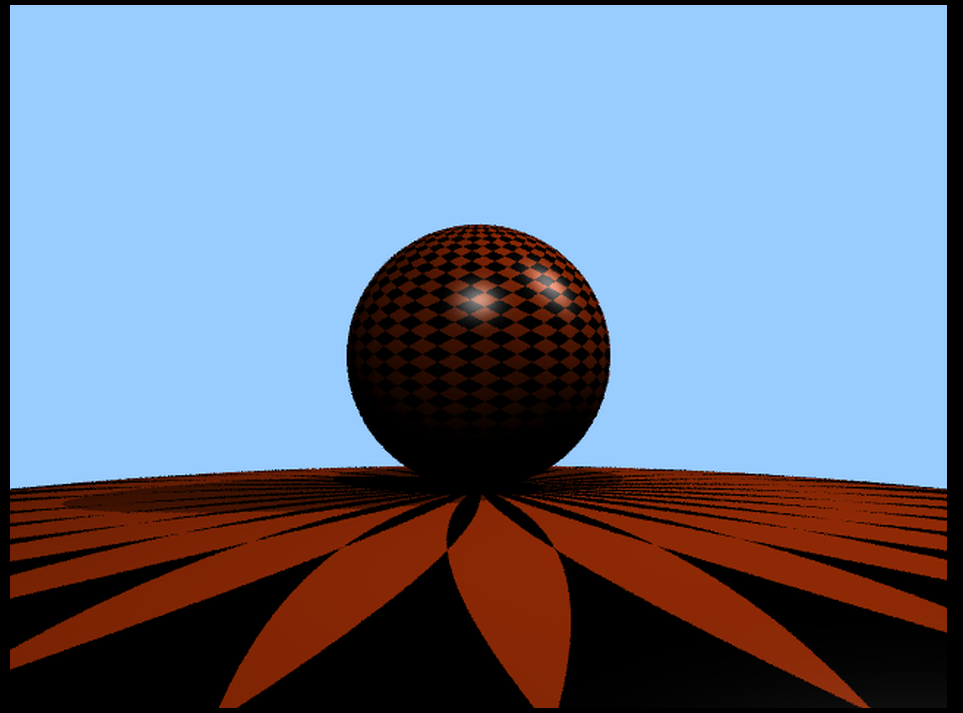
\includegraphics[width=.8\linewidth]{C:/D/University/Semester_4/Raytracer/lab_report_1/assignment_2/images/texture_1.png}  
				\caption{}
				\label{fig:sub-first}
			\end{subfigure}
			\begin{subfigure}{.3\textwidth}
				\centering
				% include second image
				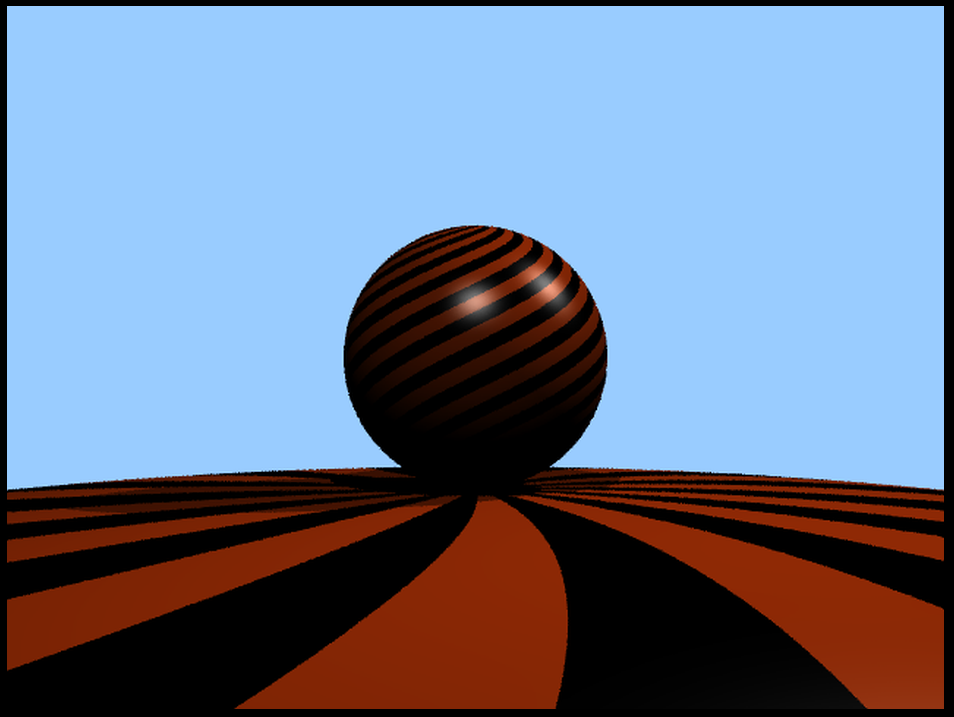
\includegraphics[width=.8\linewidth]{C:/D/University/Semester_4/Raytracer/lab_report_1/assignment_2/images/texture_2.png}  
				\caption{}
				\label{fig:sub-second}
			\end{subfigure}
			\begin{subfigure}{.3\textwidth}
				\centering
				% include second image
				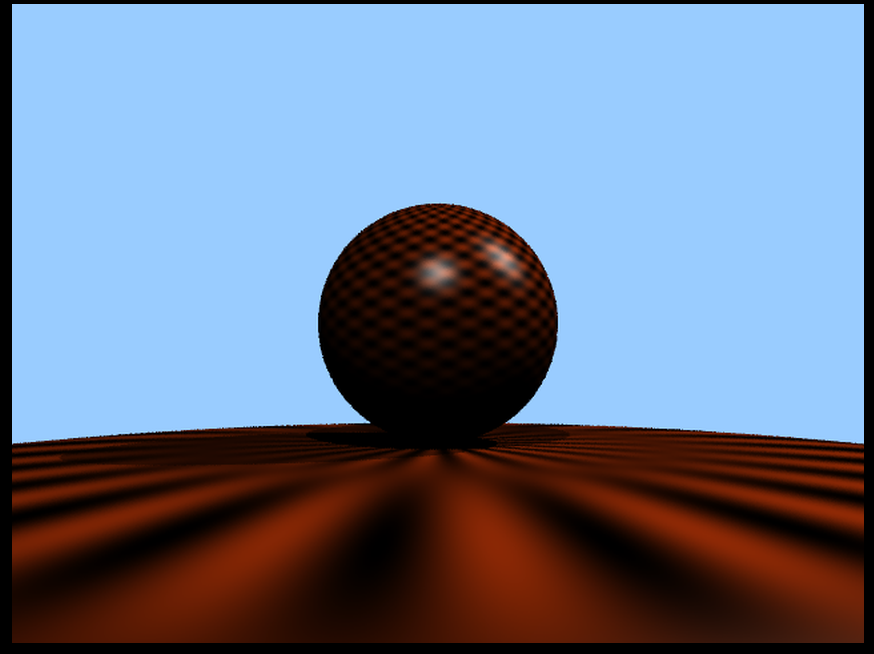
\includegraphics[width=.8\linewidth]{C:/D/University/Semester_4/Raytracer/lab_report_1/assignment_2/images/texture_3.png}  
				\caption{}
				\label{fig:sub-third}
			\end{subfigure}
			
			\caption{(a), (b) and (c) show different pattern for textures that can be generated by mathematical equations to map x and y value to different color value.}
			\label{fig:8}
		\end{center}
	\end{figure}
	
	
	\subsubsection{Results and discussion}
	Figure ~\ref{fig:9} shows the refraction phenomenon where the settings had a red glossy sphere passing behind a transparent sphere with an refractive index, $\eta$ not equal to the air we are assuming it is any kind of liqued with big $\eta$ that it refract the light with a big angle. As it can be noticed the red sphere looks larger than it should be and also inverted, moreover the ground is inverted as well, 
	\begin{figure}[H]
		\begin{center}
			\begin{subfigure}{.3\textwidth}
				\centering
				% include first image
				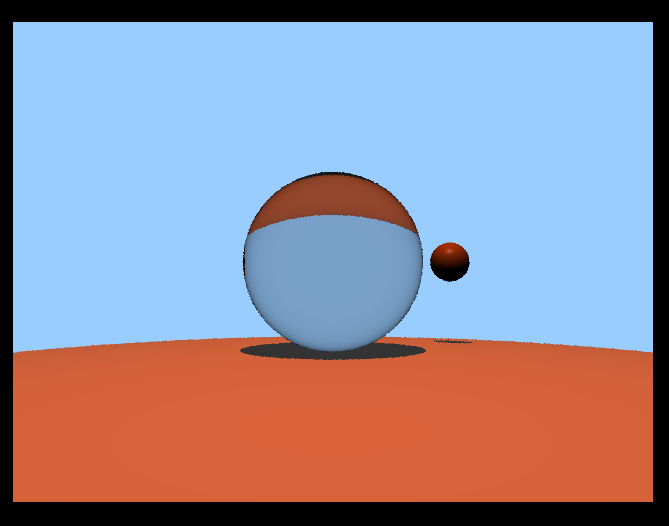
\includegraphics[width=.8\linewidth]{C:/D/University/Semester_4/Raytracer/lab_report_1/assignment_2/images/refraction_3.png}  
				\caption{ Glass sphere refracts the inverted ground upside down, the red sphere looks normal before refraction}
				\label{fig:sub-first}
			\end{subfigure}
			\begin{subfigure}{.3\textwidth}
				\centering
				% include second image
				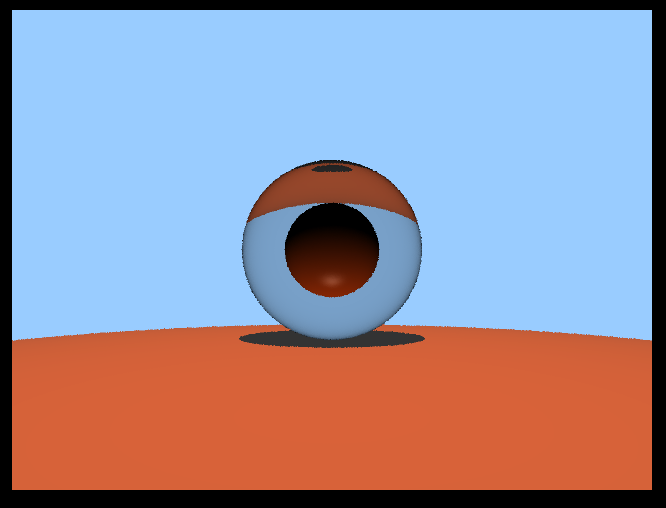
\includegraphics[width=.8\linewidth]{C:/D/University/Semester_4/Raytracer/lab_report_1/assignment_2/images/refraction_0.png}  
				\caption{The glass sphere refracts the ground, and the red Sphere directly behind it is inverted}
				\label{fig:sub-second}
			\end{subfigure}
			\begin{subfigure}{.3\textwidth}
				\centering
				% include second image
				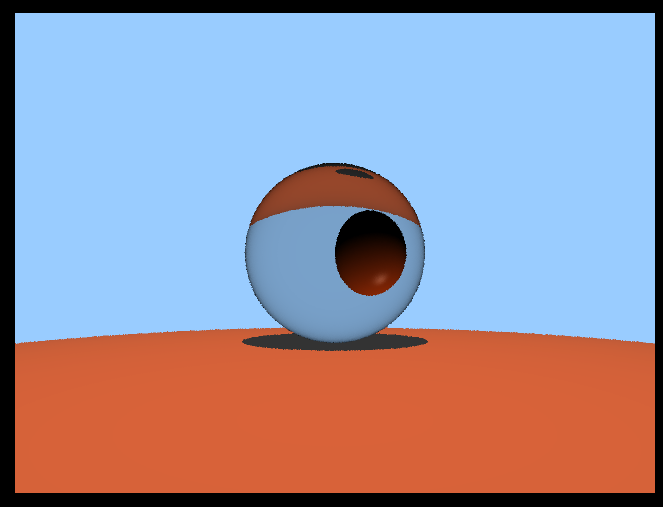
\includegraphics[width=.8\linewidth]{C:/D/University/Semester_4/Raytracer/lab_report_1/assignment_2/images/refraction__0_5.png}  
				\caption{ Glass sphere refract the ground, and red Sphere behind it inverted with an angle}
				\label{fig:sub-third}
			\end{subfigure}
			
			\caption{The scene shows a transparent sphere that refract the light, where it refract the light and shows the ground and the red sphere inverted.}
			\label{fig:9}
		\end{center}
	\end{figure}
	
	
	
	
	\textbf{Resources and further reading}: 
	Most material and code used in this chapter is mixed between the website [	Scratchapixel.com,	\textit{"Learn Computer Graphics From Scratch!"}
	] and the slides 		[Matthias Teschner, 	\textit{“Advanced Computer Graphics”}].
	\clearpage
	\section{Curves}
	\subsection{Introduction}
	We frequently need to draw different shapes and models of things onto the screen in computer graphics. Models are not always flat, and we must draw curves many times to draw a smooth model; for example, drawing the famous Utah teapot, this complex model is difficult to draw by only using triangles as the surface of the model needs a curved line than flat, straight lines. 
	
	\vspace*{5px}
	Curves have three categories: \textit{Explicit}, \textit{Implicit}, and \textit{Parametric curves}. In practice, parametric curves are used; hence in this chapter, parametric curves are used.
	
	It only requires 4 points to create a Bézier curve. These points are control points defined in 3D space. As with surfaces, the curve itself does not exist until these 4 points are combined and weighted with some coefficients. Curves defined by parametric equations have a parameter, which is a variable in this equation used to define the curve. To achieve a smoother result, increase the number of segments and points.
	Font modeling, animation, and games use curves to smooth surfaces and make the scene looks natural rather than looking edgy. 
	
	\subsection{Bézier Curves}
	They are a simple and intuitive representation of curves. They are polynomial curves represented by control points where n+1 control points are needed for a curve of degree n.
	Interpolation is used for the first and last control points; other control points are approximated. The next equation represents the control points depending on the degree n: 
	
	\begin{equation}
		\begin{split}
			\pmb{x}(t)=\sum_{i = 0}^{n} B_{i,n}(t) \pmb{P}_i, \; t \in [0,1]
		\end{split}		
	\end{equation}
	
	Where $  \pmb{P}_i $ is the set of points and $ B_{i,n}(t) $ represents the Bernstein polynomials that shown in formula 13, Where $ n $ is the polynomial degree, $ i $ is the index, and $ t  $ is the variable.
	
	
	
	\begin{equation}
		\begin{split}
			B_{i,n}(t) = \frac{n!}{(n - i)!i!}(1-t)^{n-i}t^i , \;\; 0 \leq i \leq n
		\end{split}		
	\end{equation}
	\subsection{Implementation}
	In this scenario, the curve is represented by a thin cylinder or a long string (like spaghetti).
	
	Hair rendering:
	\begin{itemize}
		\item Create Position at Regular Intervals:
		It is first necessary to create a loop of vertices along the curve and then connect these vertices together to form faces.
		\item Create a Local Coordinate System to Generate a Loop of Vertices: we will create a local coordinate system which we will need in step 3.
		
		\item Generate loop of vertices:
		It is making loops with points that are oriented correctly around curves.
		
		\item Meshing: By connecting the vertex points, we can form the faces.
	\end{itemize}	
	
	\subsection{Results and discussion}
	
	Figure ~\ref{fig:10} shows the final result after following the four points mention in the implementation, where rendering a hair as a showcase to implement curves is successful. Using more surfaces to render to cylinder makes it smoother as shown in case (a) where 16 surfaces have been used, (b) is using fewer surfaces as it uses 8, however (c) is using only 4, that is why it looks edgy. Increasing the number of surfaces depending on the quality of application; for example, for more extensive scenes, maybe choosing fewer surfaces is better to increase the performance, but for a high-quality rendering, the more surfaces, the better.
	\begin{figure}[H]
		\begin{center}
			\begin{subfigure}{.3\textwidth}
				\centering
				% include first image
				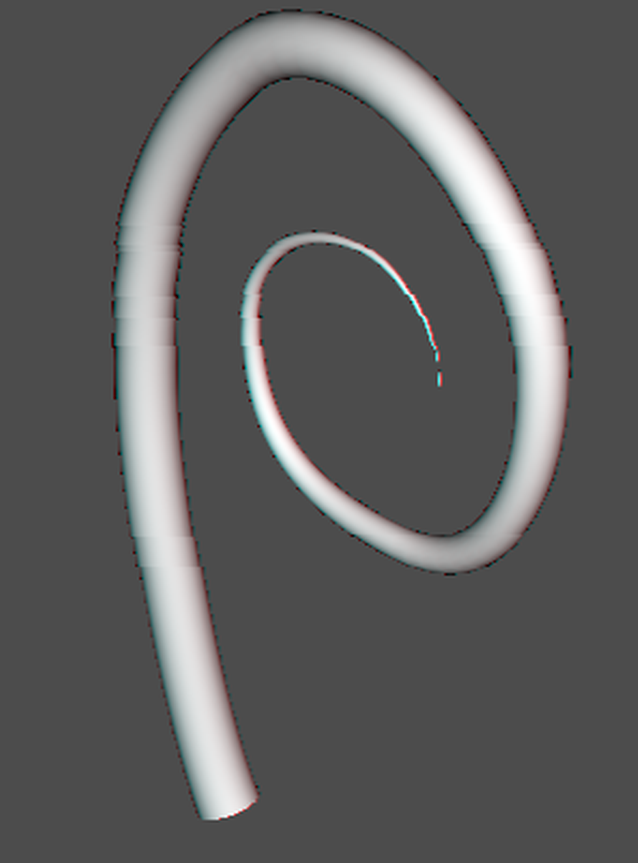
\includegraphics[width=.8\linewidth]{C:/D/University/Semester_4/Raytracer/lab_report_1/assignment_2/images/hair_n_3_div_16.png}  
				\caption{16 surfaces}
				\label{fig:sub-first}
			\end{subfigure}
			\begin{subfigure}{.3\textwidth}
				\centering
				% include second image
				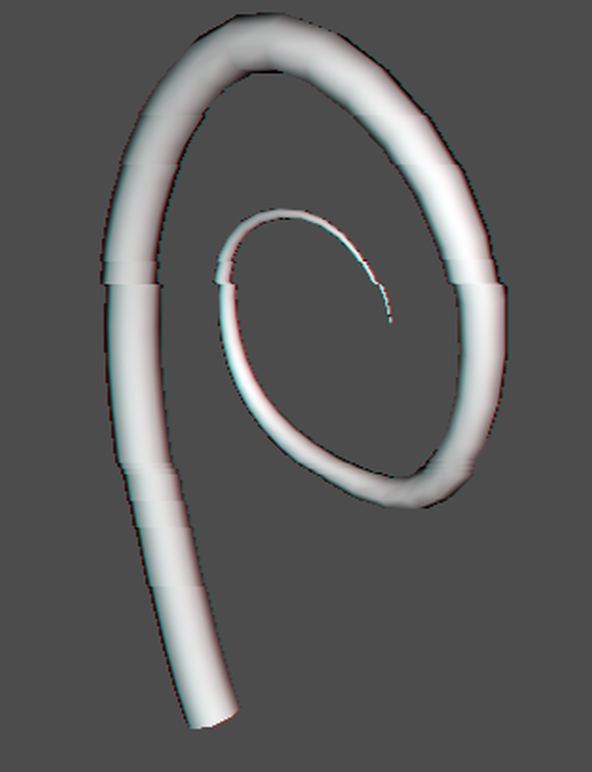
\includegraphics[width=.8\linewidth]{C:/D/University/Semester_4/Raytracer/lab_report_1/assignment_2/images/hair_n_3_div_8.png}  
				\caption{8 surfaces}
				\label{fig:sub-second}
			\end{subfigure}
			\begin{subfigure}{.3\textwidth}
				\centering
				% include second image
				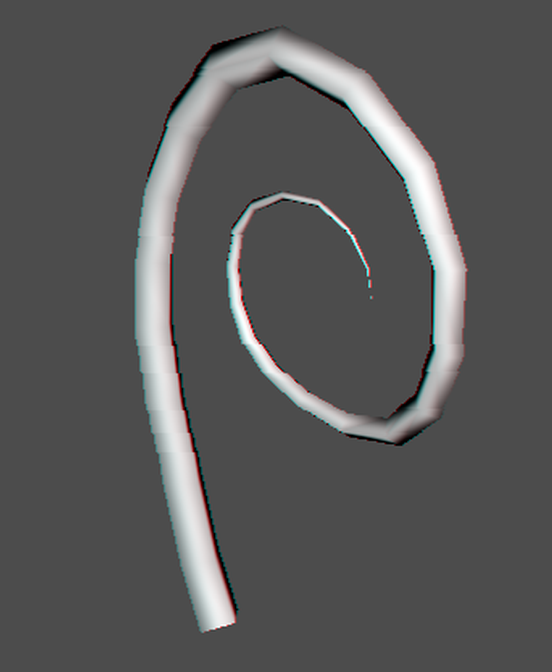
\includegraphics[width=.8\linewidth]{C:/D/University/Semester_4/Raytracer/lab_report_1/assignment_2/images/hair_n_3_div_4.png}  
				\caption{4 surfaces}
				\label{fig:sub-third}
			\end{subfigure}
			\caption{Hair rendering result for different surfaces numbers of the cylinders}
			\label{fig:10}
		\end{center}
	\end{figure}
	
	
	As mentioned before, the higher the order of the polynomial used in the Bézier Curve, the smoother the curve can be. Figure ~\ref{fig:11} shows the differences between using a polynomial of order three and two. As it can be noticed, (a) has smoother curves than (b) because (a) is using a polynomial of order three, unlike (b) that uses only two.
	\begin{figure}[H]
		\begin{center}
			\begin{subfigure}{.3\textwidth}
				\centering
				% include first image
				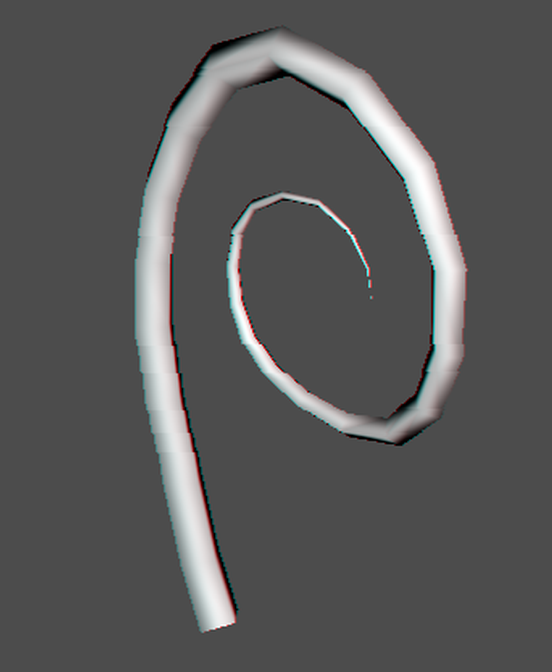
\includegraphics[width=.8\linewidth]{C:/D/University/Semester_4/Raytracer/lab_report_1/assignment_2/images/hair_n_3_div_4.png}  
				\caption{$3^{rd}$ order}
				\label{fig:sub-first}
			\end{subfigure}
			\begin{subfigure}{.3\textwidth}
				\centering
				% include second image
				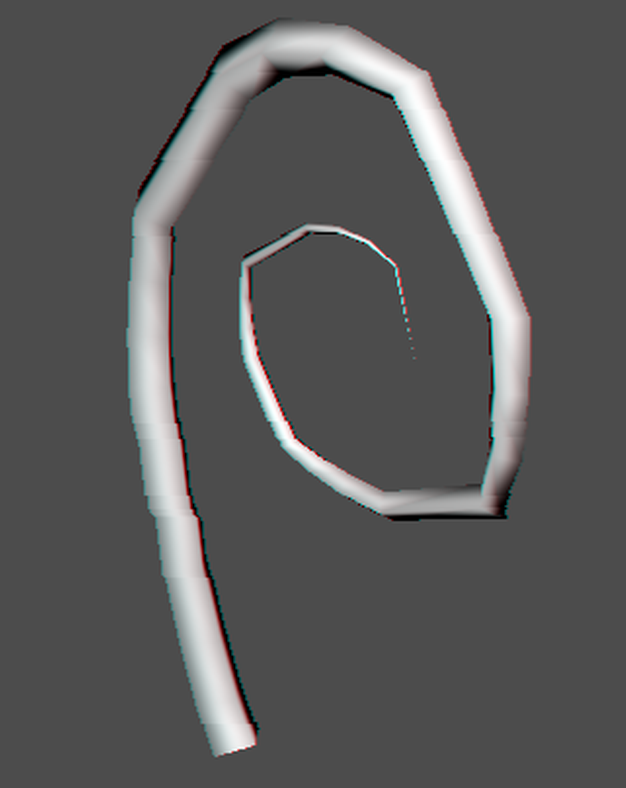
\includegraphics[width=.8\linewidth]{C:/D/University/Semester_4/Raytracer/lab_report_1/assignment_2/images/hair_n_2_div_4.png}  
				\caption{$2^{nd}$ order}
				\label{fig:sub-second}
			\end{subfigure}
			\caption{Hair rendering result for different polynomial order.}
			\label{fig:11}
		\end{center}
	\end{figure}
	
	\textbf{Resources and further reading}: 
	Most material and code used in this chapter is mixed between the book [Peter Shirley. 	\textit{"Ray Tracing in One Weekend"}] and the slides 		[Matthias Teschner, 	\textit{"Advanced Computer Graphics"}].
	
	
	\clearpage
	\section{Bounding Volume Hierarchies - BVH}
	\subsection{Introduction}
	\label{definitions}
	Bounding Volume Hierarchies, known as "BVH," is simply a data structure representing complex geometric models with specific simple bounding volumes to reduce some of the expensive tests in different computer graphics applications.
	BVH is object-oriented, unlike other algorithms such as kd-trees which are space subdivisions.
	
	
	
	
	\subsection{Motivation}
	There are two main applications for bounding volume hierarchy, in retracing where two main challenges have to be solved: Shading and visibility; usually the Raytracer has to test each model in the scene in order to render it to the screen, on the other hand, some of the models they are not visible to the camera and testing them make no sense therefore by telling the rays which models to test the intersection this will boost the performance of the Raytracer tremendously, BVH can quickly achieve this.
	
	Moreover, the collision detection algorithm used in simulation and games can benefit significantly from BVH.
	
	\subsection{Bounding volume - BV}
	Bounding volume is the tightest possible virtual volume that wraps up a model in a scene. It is the fundamental component that builds the BVH tree.
	
	There are four different main types of BV depending on the shape complexity:
	
	\begin{itemize}
		\item Spheres.
		\item Axis Aligned Bounding Box (AABB).
		\item Oriented Bounding Box (OBB).
		\item Discrete Oriented Polytope (k-DOP).
	\end{itemize}	
	\subsection{BVH Tree construction}
	Nodes in the BVH tree are BV, and leaves are primitives. 
	There are three different ways to construct a BVH tree:
	\begin{itemize}
		\item Top Down:	Arguably the most popular technique in practice. It uses the 'fit and split' algorithm, where it starts with the whole model and encapsulates it with a BV and fits it, then tries to split it into n children, usually 2. It keeps recursively splitting and fitting until it reaches the leaves and assigns the primitives to them.
		
		\item Bottom Up: Slower construction time than Top-Down but usually produces the best tree. It uses the 'knit and fit' algorithm, where it starts with primitives and tries to encapsulate them with the BV and merge each n, usually n=2; it keeps recursively doing this process until it reaches the root.
		
		
		\item Insertion: It uses 'incremental-insertion' algorithm, where it starts with a single leaf and merges another leaf by using a cost function, then creating a head node and searching for the next leaf to merge. The problem with this method is that it can become worst as it depends on the insertion order of the nodes, and it is challenging to find the best tree.
		
	\end{itemize} 
	
	\subsection{Implementation}
	
	In this Raytracer, a Sphere BV is used; the reason is simple as Sphere has a fast intersection test and is easy to generate and fit into the model or primitives. 
	On the other hand, Sphere is usually not so tight, resulting in non-optimal performance, but for this Raytracer, as the scene is not significant and complex, Spheres can be a good choice.
	
	For constructing the BVH tree, the Bottom-Up method is used. Moreover, a binary tree and minimum leaves = 2 are the settings.
	
	\subsection{Results and discussion}
	
	Figure ~\ref{fig:12} (a) shows eight particles that will be used as a test scene; these particles are the leaves in our tree that present layer 4. Because we are using a bottom-up strategy, every two particles are merged and encapsulated by one Sphere BV. This creates a higher level of the tree, layer 3. Recursivity we keep merging every two BVs until we hit the root, as shown in (d).
	
	\begin{figure}[ht]
		\begin{center}
			\begin{subfigure}{.3\textwidth}
				\centering
				% include first image
				\includegraphics[width=.8\linewidth]{C:/D/University/Semester_4/Raytracer/lab_report_1/assignment_2/images/bvh/l4.png}  
				\caption{Level 4: Particles that will be encapsulate by BV}
				\label{fig:sub-first}
			\end{subfigure}
			\begin{subfigure}{.3\textwidth}
				\centering
				% include second image
				\includegraphics[width=.8\linewidth]{C:/D/University/Semester_4/Raytracer/lab_report_1/assignment_2/images/bvh/l3.png}  
				\caption{Level 3: Sphere BV wraps up particles}
				\label{fig:sub-second}
			\end{subfigure}
			\begin{subfigure}{.3\textwidth}
				\centering
				% include second image
				\includegraphics[width=.8\linewidth]{C:/D/University/Semester_4/Raytracer/lab_report_1/assignment_2/images/bvh/l2.png}  
				\caption{Level 2: Second level of the BVH tree}
				\label{fig:sub-third}
			\end{subfigure}
			\begin{subfigure}{.3\textwidth}
				\centering
				% include second image
				\includegraphics[width=.8\linewidth]{C:/D/University/Semester_4/Raytracer/lab_report_1/assignment_2/images/bvh/l1.png}  
				\caption{Level 1: This is the root node the cover all the BVs and particles}
				\label{fig:sub-forth}
			\end{subfigure}
			\caption{BVH result when a Sphere BV used and the scene is eight particles}
			\label{fig:12}
		\end{center}
	\end{figure}
	
	In order to test the BVH performance, three main tests have been done. Table 1 illustrates the differences between using BVH or not. By looking into the table, we noticed that using the BVH spends double the time of not using BVH. The main reason is that BVH adds more steps to the Raytracer; it adds tree Construction cost and adds BV generation cost. BVH is useful when more extensive scenes are used; for example, by including 16 particles in the scene and excluding the other 16 particles from the camera vision, we can see that BVH boosts the Raytracer's performance.
	
	\begin{table}[h!]
		\centering
		\begin{tabular}{||c c c c||} 
			\hline
			- & 8/8  & 16/16 & 16/32 \\ [0.5ex] 
			\hline\hline
			With BVH & 7s & 10s & 10s \\ 
			\hline
			Without BVH & 3s & 7s & 12s \\
			\hline
			
		\end{tabular}
		\caption{The Raytracer performance comparison, where 16/32 means 32 particles are used in the sceen and only 16 are included in the image.}
		\label{table:1}
	\end{table}
	
	
	\clearpage
	
	\section{Summary and conclusion}
	In the first chapter, Visibility, we introduced different shapes that can be represented in the 3D scene; it can be noticed that some are easier to be rendered than others depending on how complex the model is, but also the intersection test plays a considerable role for the performance. Also, some complex shapes like tetrahedra and cubes can be reconstructed by building up a trivial model as triangles.  
	
	Moreover, rendering pixels can lead to aliasing where the edges of the model look sharp and not realistic; this can be solved by using different anti-aliasing methods; however, this can reduce the performance of the Raytracer.
	
	The Shading chapter Phong model is used to approximate the light effect on Spheres where diffuse and glossy models are used; also, different materials such as transparent have been implemented and shown using snells law. Textures are a simple method to shade a model without using expensive operations, and a math model can give excellent results. 
	
	In Shading, the more Rays paths are followed for rendering, the more realistic the scene becomes; however, the deeper we trace the Rays, the more expensive the Raytracer becomes as it needs more paths to trace. 
	
	Curves are not trivial to be approximated in computer graphics because we approximate curves by lines; hence, the smoother the curve, the more lines are needed. As we introduced the polynomials, if we want a complex curve, we need a higher-order polynomial, which leads to higher memory consumption and reduces the Raytracer's performance. 
	
	As ray tracing operations are expensive and more paths to be traced, some data structures are used to increase the Raytracer performance and efficiency, some methods are space subdivisions as kd-trees, and others objects originated as BVH. BVH can reduce the number of intersection tests needed; however, it adds more steps to the workflow as tree construction, updates, and traversal.  BVH can be optimized by tweaking the BV types used, tree construction algorithms, and traversal algorithms.
	
	In this report, different resources are used for the implementation to search and test different approaches of Raytracer.  The report illustrates the basic approaches and challenges that can encounter the engineer to solve the rendering challenge. 
	
	
	\clearpage
	%----------------------------------------------------------------------------------------
	%	BIBLIOGRAPHY
	%----------------------------------------------------------------------------------------
	
	\begin{thebibliography}{9}
		\bibitem{latexcompanion} 
		Fangkai Y. 	\textit{"Collision Detection in Computer Games"}. KTH Royal Institute of Technology.
		
		\bibitem{latexcompanion} 
		Hamzah S, Abdullah B. 	\textit{"Bounding Volume Hierarchies for Collision Detection"}
		
		\bibitem{latexcompanion} 
		Matthias Teschner, 	\textit{“Advanced Computer Graphics”}, University of Freiburg.
		
		\bibitem{latexcompanion} 
		Matthias Teschner, 	\textit{“Simulation in Computer Graphics Bounding Volume Hierarchies”}, University of Freiburg.
		
		
		\bibitem{latexcompanion} 
		Peter Shirley. 	\textit{“Ray Tracing in One Weekend”}
		
		\bibitem{latexcompanion} 
		Peter Shirley. 	\textit{“Ray Tracing: The Next Week”}
		\bibitem{latexcompanion} 
		Piotr Dubla. 	\textit{"Interactive Global Illumination on the CPU"}
		
		\bibitem{latexcompanion} 
		Scratchapixel.com,	\textit{"Learn Computer Graphics From Scratch!"}
		
		
		\bibitem{latexcompanion} 
		Stefan G.	\textit{"Collision queries using bounding box"}. The University of North Carolina.
		
		
		
		
	\end{thebibliography}
	%----------------------------------------------------------------------------------------
	
	
\end{document}